\documentclass[tikz,border=10pt]{standalone}
\usepackage[T1]{fontenc}
\usepackage{lmodern}
\usetikzlibrary{arrows.meta,calc}
\newcommand{\boxtitle}[1]{{\bfseries #1}\\[5pt]}
\begin{document}
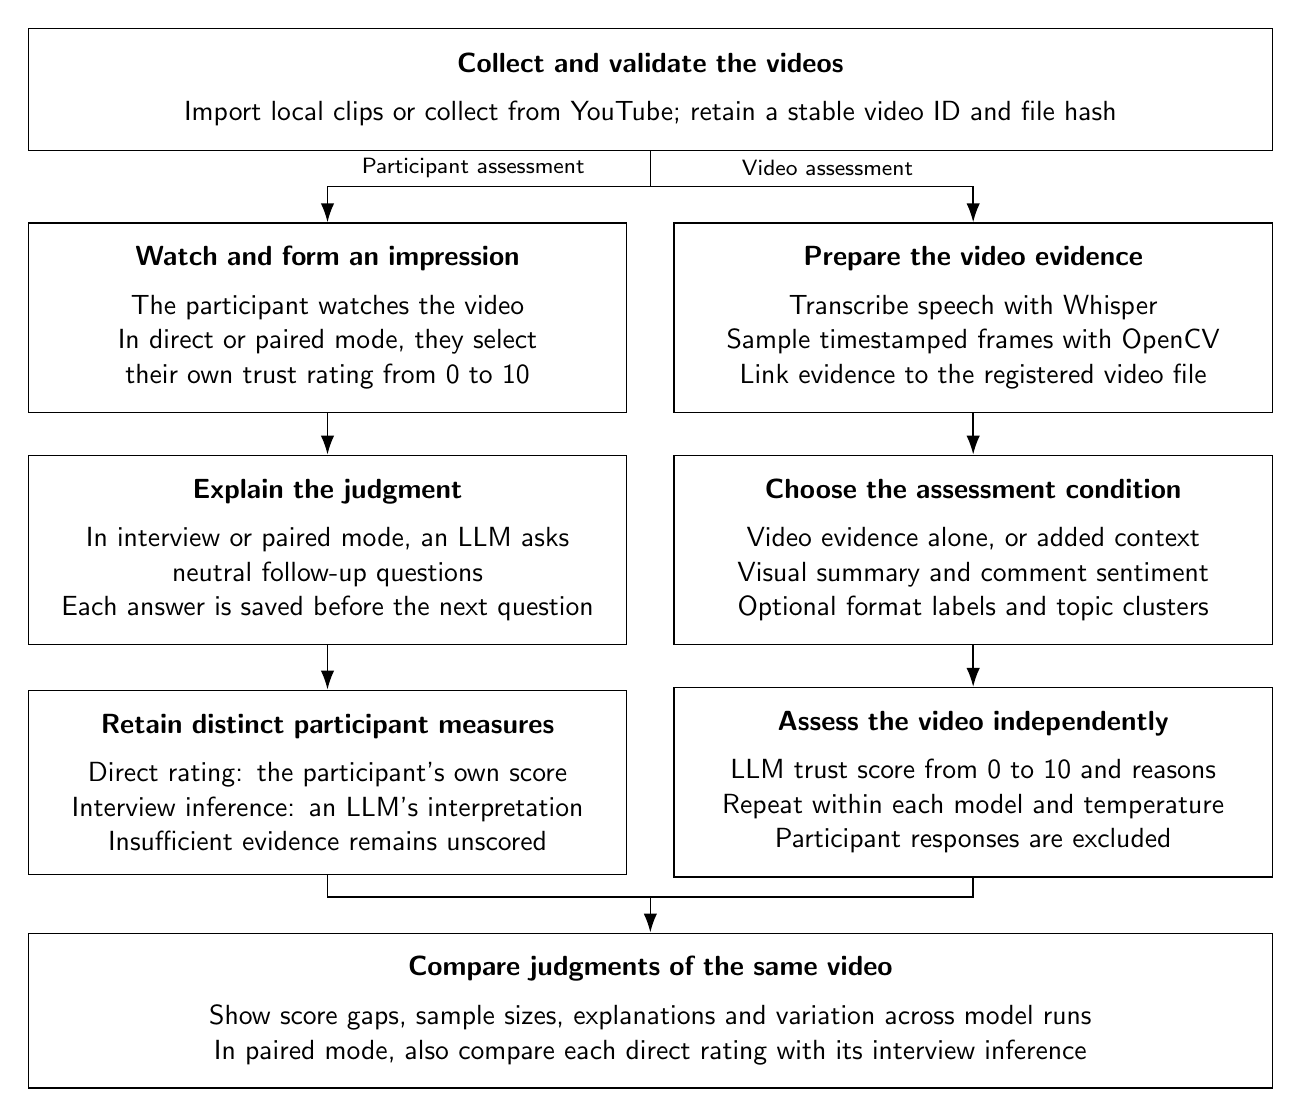
\begin{tikzpicture}[
    font=\sffamily\fontsize{10}{12.5}\selectfont,
    box/.style={rectangle,draw=black,fill=white,line width=0.45pt,
        text width=6.8cm,minimum height=2.25cm,
        inner xsep=4mm,inner ysep=3mm,align=center},
    wide/.style={box,text width=15cm,minimum height=1.55cm},
    line/.style={draw=black,line width=0.6pt},
    arrow/.style={line,-{Latex[length=2.4mm,width=1.7mm]}},
    branchlabel/.style={font=\sffamily\footnotesize,fill=white,inner sep=2pt}
]
\node[wide] (videos) at (0,0) {
    \boxtitle{Collect and validate the videos}
    Import local clips or collect from YouTube; retain a stable video ID and file hash
};
\node[box] (watch) at (-4.1,-2.9) {
    \boxtitle{Watch and form an impression}
    The participant watches the video\\
    In direct or paired mode, they select\\their own trust rating from 0 to 10
};
\node[box] (interview) at (-4.1,-5.85) {
    \boxtitle{Explain the judgment}
    In interview or paired mode, an LLM asks\\neutral follow-up questions\\
    Each answer is saved before the next question
};
\node[box] (participant) at (-4.1,-8.8) {
    \boxtitle{Retain distinct participant measures}
    Direct rating: the participant's own score\\
    Interview inference: an LLM's interpretation\\
    Insufficient evidence remains unscored
};
\node[box] (content) at (4.1,-2.9) {
    \boxtitle{Prepare the video evidence}
    Transcribe speech with Whisper\\
    Sample timestamped frames with OpenCV\\
    Link evidence to the registered video file
};
\node[box] (context) at (4.1,-5.85) {
    \boxtitle{Choose the assessment condition}
    Video evidence alone, or added context\\
    Visual summary and comment sentiment\\
    Optional format labels and topic clusters
};
\node[box] (model) at (4.1,-8.8) {
    \boxtitle{Assess the video independently}
    LLM trust score from 0 to 10 and reasons\\
    Repeat within each model and temperature\\
    Participant responses are excluded
};
\node[wide] (compare) at (0,-11.7) {
    \boxtitle{Compare judgments of the same video}
    Show score gaps, sample sizes, explanations and variation across model runs\\
    In paired mode, also compare each direct rating with its interview inference
};
\coordinate (split) at ($(videos.south)+(0,-0.45)$);
\draw[line] (videos.south) -- (split);
\draw[arrow] (split) -| (watch.north);
\draw[arrow] (split) -| (content.north);
\path (split) ++(-2.25,0.23) node[branchlabel] {Participant assessment};
\path (split) ++(2.25,0.23) node[branchlabel] {Video assessment};
\draw[arrow] (watch.south) -- (interview.north);
\draw[arrow] (interview.south) -- (participant.north);
\draw[arrow] (content.south) -- (context.north);
\draw[arrow] (context.south) -- (model.north);
\coordinate (merge) at ($(compare.north)+(0,0.45)$);
\draw[line] (participant.south) |- (merge);
\draw[line] (model.south) |- (merge);
\draw[arrow] (merge) -- (compare.north);
\end{tikzpicture}
\end{document}
